This chapter will aim to cover background knowledge about the LLVM Framework and features of a wide SIMD. After that the related work follows, which discusses other exposed or explicit datapath architectures, the legacy compiler and developments on the LLVM-based compiler for the target SIMD architecture.

\section{LLVM Compiler Framework}\label{sec:llvm}
%TODO: add LLVM-IR example/CFG picture, etc.

The LLVM project was started in 2000 by Chris Lattner, as a research project at the University of Illinois with the goal of providing a modern, \emph{Static Single Assignment} (SSA)-based compilation strategy capable of supporting both static and dynamic compilation of arbitrary programming languages. It was first released in 2003 and the project has grown rapidly since then. It has become popular amongst major companies, e.g. Google, Apple, and Sony, for its powerful multi-stage compilation strategy and outstanding extendability. LLVM is a collection of modular and reusable compiler and toolchain technologies. Generally, LLVM follows a 3-phase design, which is divided between a frontend, a code independent optimizer and a backend, illustrated in Figure \ref{fig:3phase_design}.

\begin{figure}[H]
\centering
\includegraphics[width=.75\textwidth]{figures/3phase_design}%
\caption{3-phase design: frontend, optimizer and backend.}
\label{fig:3phase_design}
\end{figure}

%TODO: Reorder list: [IR, Lexical analysis, Syntax analysis, ]
\textbf{The frontend} is responsible for translating code of an arbitrary programming language into LLVM's \emph{Intermediate Representation} (IR) code. The LLVM instruction set represents a virtual architecture that captures the key operations of ordinary processors, but avoids machine specific constraints such as physical registers. Instead, it has an infinite amount of virtual registers in SSA form, which means that each virtual register is assigned only once and each use of a variable is dominated by that variable's definition. This simplifies the data flow optimizations because only a single definition can reach a particular use of a value, and to find that definition is trivial \cite{llvm_strategy}.

%\begin{lstlisting}[caption=Bundled instructions.,frame=tlrb]{ir_c}
%
%\end{lstlisting}

%TODO discuss of this example with phi should be in there? is it usefull? think not
%\captionof{lstlisting}{Fragment of code with a phi instruction.}
%\begin{center}
%\hspace{2px}\begin{minipage}{.475\textwidth}
%\lstset{style=customc}
%\begin{lstlisting}[caption=List of instructions.,frame=tlrb]
%\begin{lstlisting}[frame=tlrb]
%int foo(int a, int b)
%{
%  if (a > b)
%    return a;
%  else
%    return b;
%}
%
%
%
%
%
%
%<@\ @>
%\end{lstlisting}
%\end{minipage}\hfill
%\begin{minipage}{.475\textwidth}
%\lstset{style=customasm}
%%\begin{lstlisting}[caption=IR-code.,frame=tlrb]
%\begin{lstlisting}[breaklines, frame=tlrb]
%define i32 @foo(i32 %a, i32 %b) #0 {
%entry:
%  %cmp = icmp sgt i32 %a, %b
%  br i1 %cmp, label %if.then, label    %if.else
%if.then:
%  br label %return
%if.else:
%  br label %return
%return:
%  %retval.0 = phi i32 [ %a, %if.then ], [ %b, %if.else ]
%  ret i32 %retval.0
%}
%\end{lstlisting}
%%\vspace{1.9em}
%\end{minipage}
%\end{center}

%frontend talk, straight from the Dragon Book plz.
%introduce parser and lexical analysis and that it is kept in an AST, which will be translated as a final step to IR.
%Perhaps an example?
%TODO: rewrite first sentence in my own words.
Figure \ref{fig:frontend} gives an overview of a frontend. The main task of the lexical analyzer is to read the input characters of the source program, group them into luxemes, and produce as output a sequence of tokens. These tokens are used by the parser for syntax analysis, where it is verified that the sequence of tokens can be reconstructed according to the syntax of the input language. The parser reports any syntax errors during this process and should be able to recover from the error in order to continue processing the rest of the program. The parser constructs a parse tree, and the semantic analyzer uses this parse tree to check for consistency with the language definition. Type checking is also done during this stage, and the information is kept in a syntax tree. The result of these phases is an \emph{Abstract Syntax Tree} (AST) of the program, which can be translated into three-address IR code. %We will discuss LLVM's IR in more detail in Chapter \ref{sec:ir}

\begin{figure}[t]
\centering
\includegraphics[width=\textwidth]{figures/frontend}%
\caption{Overview of the components that the frontend compromises.}
\label{fig:frontend}
\end{figure}

Listing \ref{lst:ir_code} shows an example C code where where we multiply two arguments and add them together to a third argument. On the right-hand part of this listing we can see the output that is generated by the front-end. Here we already have a notion of labels, similar to that of assembly code. The LLVM-IR code is in SSA form and consists of three-address operations. Here \emph{nsw} indicates that the result is undefined in case of an overflow.
%TODO BIG: add reference to 2.1, tell something about llvm's ir code representation, give examples, show phi node. 

\captionof{lstlisting}{Fragment of C code with corresponding LLVM-IR.}\label{lst:ir_code}
\begin{center}
\hspace{2px}\begin{minipage}{.475\textwidth}
\lstset{style=customc}
%\begin{lstlisting}[caption=List of instructions.,frame=tlrb]
\begin{lstlisting}[frame=tlrb]
int foo(int a, int b, int c)
{
  c += a*b;
  return c;
}

<@\ @>
\end{lstlisting}
\end{minipage}\hfill
\begin{minipage}{.475\textwidth}
\lstset{style=customasm}
%\begin{lstlisting}[caption=IR-code.,frame=tlrb]
\begin{lstlisting}[frame=tlrb]
define i32 @foo(i32 %a, i32 %b, 
                i32 %c) #0 {
entry:
  %mul = mul nsw i32 %b, %a
  %add = add nsw i32 %mul, %c
  ret i32 %add
}
\end{lstlisting}
%\vspace{1.9em}
\end{minipage}
\end{center}

% TODO: make graph to categorise optimizations on some criteria
\textbf{The optimizer} contains a collection of analysis and semantic-preserving transformations that can be used to optimize IR code. One of the advantages of LLVM is that when you build a new backend for any given processor architecture you immediately have access to all of these optimizations. Below we give some of these optimizations that are explained more detailed in the literature \cite[Chapter~9]{dragon_book}.%TODO: fix chapter in cite.
%TODO: add mem2reg
\begin{itemize}
\item \emph{Constant propagation:} computes for each point and each variable in the program, whether that variable has a unique constant value at that point. This can then be used to replace variable references with constant values.
\item \emph{Constant folding:} recognizes and evaluates constant expressions at compile time rather than runtime. For example, `$add\ 1+2$' can be replaced by `$3$'. Statements like `$add\ 1+2$' can be introduced by other optimizations, e.g. constant propagation. 
\item \emph{Common sub-expression elimination:} recognizes that the same expression appears in more than one place, and that performance can be improved by transforming the code such that the expression appears in one only place.
\item \emph{Copy propagation:} replaces each target of a copy statement with that of the copied value. For example, if we have a copy statement, $x = y$. Then the uses of $x$ can be replaced by $y$. Some optimizations require that this optimization is performed afterward to clean up, e.g. common sub-expression elimination requires this pass to run afterward. 
\item \emph{Dead code elimination:} removes code that does not affect the program's results. This avoids executing irrelevant operations and reduces the code size of a program.  
\item \emph{Loop invariant code motion:} aims at moving code that is independent of the loop iteration out of the loop body. It does this by moving the loop independent statement above the loop, saving it in a temporary variable, and use it in each iteration of the loop. Now the loop independent statement is computed only once instead of every iteration. 
\item \emph{Function inlining:} verifies whether inlining functions in its callees gives a performance benefit. If doing this would give a performance benefit, it replaces the call to the function with the function body. This optimization often is useful for small functions because it reduces the overhead that is introduced when a function call is made, e.g. storing frame pointer, storing function parameters and jump to the code to where the function is defined.     
\end{itemize}

\begin{figure}[b!]
\centering
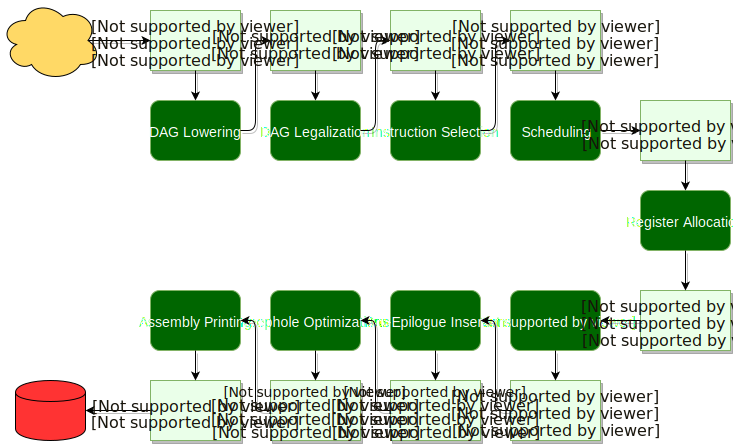
\includegraphics[width=\textwidth]{figures/code_generation_sequence}%
\caption{Code generation sequence, from LLVM code to assembly code.}
\label{fig:code_generation}
\end{figure}

%TODO: apply following namings: Instruction, Machine instruction, scheduled instruction in SSA form, schedule instruction not in SSA form.
\textbf{The backend} translates, according to a processor architecture, IR code to a target specific assembly language. It does this by going through a sequence of code generation stages, illustrated in Figure \ref{fig:code_generation}. The rectangular boxes indicate the data structure that is used by and produced by a given stage, and the name of each stage is denoted in a rectangular box with rounded corners. During this process, first, the IR code is lowered to a \emph{Directed Acyclic Graph} (DAG) in which each node represents an instruction. However, for some architectures, not all data types and instructions are supported. For this reason, the DAG is legalized to something that is supported by the target architecture. Instruction selection maps each of the nodes onto machine nodes, by matching patterns. %After that, the instruction selector maps the pattern of LLVM code into the target machine code and builds a new DAG whose nodes represents the target instructions.
Then we have a DAG consisting of only target specific machine instructions, in SSA form. Having naive machine instructions, the next step is to schedule them. We schedule the machine instructions according to the resource information of the target processor and assign each instruction to a specific cycle. 
%We will discuss scheduling in more detail in Chapter \ref{sec:scheduling}. 
Now the instructions are represented in a list rather than a DAG, but still in SSA form. The \emph{Register Allocator} (RA) then assigns physical registers to each of the virtual registers, now the list is not in SSA form. 
%We will discuss RA in more detail in Chapter \ref{sec:register_allocation}. 

The post-allocation pass can improve the schedule by taking physical registers and register pressure, that is known at this point, into account. After that, some epilogue and prologue code may be inserted, for example, saving/restoring the caller/callee registers and reserving/destroying of the function's stack frame. Peephole optimizations are target specific improvements to the generated code. These optimizations deal with very specific optimizations that can only be done at the end of the process. Finally, the assembly printer prints the generated code to a file.
%backend talk -> huuge



%\subsection{Instruction Scheduling}\label{sec:scheduling}
%After instruction selection, the program is represented in SSA form as a DAG. Each instruction is represented as a $MachineSDNode$ in a $MachineBasicBlock$. After scheduling has been performed, each instructions now is represented as a $MachineInstr$. 



%ach instruction is scheduleDuring instruction schdduling, each $MachineBasicBlock$ is scheduled by the scheduler and transformed into a $MachineInstr$. After this phase, instructions are represented as $MachineInstr$.

%\subsection{Register Allocation}\label{sec:register_allocation}
%Register allocation is executed during the code generation phase and consists of finding a mapping of a program with an unlimited number of virtual registers to a program with a limited number of physical registers.
%Examples, machine instrs on the left in SSA form, on the right with proper registers next to it.
%Introduce at least 

%TODO: 19 sept morning, Add examples of IR, CFG, Dominator tree ettc.
\subsection{Control Flow}\label{sec:control_flow_graph}
%\subsection{Representation of Code}
To analyze a code fragment, different representations can be explored. For instance, three-address IR code that is used by LLVM is conducive for further processing like optimizations and translations. Even further down the compilation line, we have assembly code, which is basically object code, but in human readable form. However, to analyze a fragment of code, we do not always need this much detail. Moreover, having this much detail, sometimes makes analysis more difficult. Control flow analysis is a code technique to analyze the control flow of a program. The control flow is expressed as a \emph{Control Flow Graph} (CFG), which is a more abstract representation of code that uses a graph notation to show all paths that can be traversed through a program during its execution.  
%TODO: Add cfg example with code left, cfg right

\begin{figure}[H]
\centering
\subfloat[C code fragment]{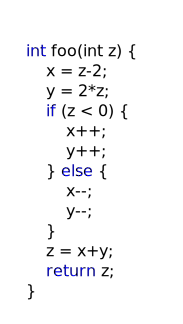
\includegraphics[width=.2\textwidth]{figures/cfg_fragment}%
\label{fig:cfg_fragment}}\quad\quad
\subfloat[CFG]{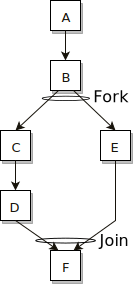
\includegraphics[width=.175\textwidth]{figures/cfg_fork_join}%
\label{fig:cfg_graph}}
\hfill
\caption{Example CFG with C code.}
\label{fig:cfg}
\end{figure}

In Figure \ref{fig:cfg_graph} we see a CFG for the code fragment in Figure \ref{fig:cfg_fragment}. In a CFG edges represent the control flow of the program and nodes represent basic blocks. A \emph{Basic Block} (BB) is a sequence of instructions with no branches, except for entering and leaving the basic block.



%Another code representation that we would like to discuss here is a Dominator Tree (DomTree). Similar to a CFG, nodes represent BBs, but edges represent a dominator relationship. For two nodes $A$ and $B$, we say that $A$ dominates $B$, if all paths to $B$ go through $A$.

%TODO: add example CFG with corresponding DomTree

\subsection{Data Dependencies and Spilling}\label{sec:data_dependencies}
%\subsection{Scheduling Constraints}\label{sec:scheduling_and_ra}
%As we have seen above,
From a compilers perspective, certain operations address memory locations. A \emph{store} operation accesses the memory to put the value of a register into memory at a certain location, addressable by its address. On the other hand, \emph{load} operations load a value from memory at a certain location and puts that value in a register. These kind of operations are called memory operations. Other operations calculate a value and stores the result in a register. Operations that store the result in a register, or load a value from memory into a register, actually define that register. An example is given in the following code fragment:

%\lstset{style=customasm}
\begin{lstlisting}
lw  r2, r0, 4   # load from memory at location 0x4
lw  r3, r0, 5   # load from memory at location 0x5
mul r3, r3, r2  # define r3 with r3 = r3 * r3
sw  r3, r0, 2   # store result at location 0x2
\end{lstlisting}

Before scheduling and register allocation, the sequence of instructions contain an unlimited number of virtual registers and the instructions are in a DAG that preserves all control flow and data dependencies. Data dependencies are ordering constraints that influence the order of execution. Typically, there are three kinds of data dependencies \cite{data_dependece}:
\begin{enumerate}
\item There is a Read-after-Write (RaW) dependency, also called a \emph{flow dependency} from operation $a$ to operation $b$ if $a$ defines a register that may be used by $b$.
\item  There is a Write-after-Read (WaR) dependency, also called an \emph{anti-dependency} if for operations $a$ and $b$ when $a$ uses a register that is redefined by $b$. 
\item There is a Write-after-Write (WaW) dependency, or \emph{output dependency} from operation $a$ to operation $b$, if $a$ defines a register that is redefined by $b$.
\end{enumerate} 

Flow dependencies are also known as \emph{true dependencies} and anti and output dependencies as \emph{false dependencies}, introduced by scheduling or register allocation. While in SSA form, each variable is defined exactly once, therefore, we have only true dependencies in that form. After scheduling and register allocation, where we assign physical registers to each virtual register, we may assign one physical register to multiple virtual registers, which is illustrated in Listing \ref{lst:ra_example}. This process introduces false dependencies and can often be resolved with renaming techniques \cite{tta_codegen,renaming}.

\captionof{lstlisting}{Redefining physical registers by assigning them to multiple virtual registers.}
\begin{center}
%TODO: include a data dependency graph for the example below
\hspace{2px}\begin{minipage}[t]{.475\textwidth}
\begin{lstlisting}[frame=tlrb]
mul %v1, %src1, %src2
add %v2, %1,    %sum
mul %v3, %src3, %src4
add %v4, %v2,   v3
\end{lstlisting}
\end{minipage}\hfill
\begin{minipage}[t]{.475\textwidth}
\begin{lstlisting}[frame=tlrb]
mul r1, r5, r6
add r2, r1, r21
mul <@\hspace{1px}\textcolor{red!70!black}{r1}\hspace{1px}@>, r7, r8  # redefines r1
add <@\hspace{1px}\textcolor{red!70!black}{r2}\hspace{1px}@>, r2, r1  # redefines r2
\end{lstlisting}
\end{minipage}
\label{lst:ra_example}
\end{center}

%\lstset{style=customasm}
%\begin{center}
%\begin{minipage}{\linewidth}
%      \centering
%      \begin{minipage}{0.45\linewidth}
%          \begin{lstlisting}[frame=tlrb]
%(a) lw  r2, r5, 4
%(b) lw  r3, r6, 6
%(c) mul r3, r3, r2
%(d) lw  r4, r7, 0
%(e) add r4, r3, r4
%(f) sw  r4, r11, 0
%\end{lstlisting}
%          \captionof{subfigure}{Assembly code}
%          \label{fig:ddg_fragment}
%      \end{minipage}
%      \begin{minipage}{0.45\linewidth}
%          \begin{figure}[H]
%          \centering
%              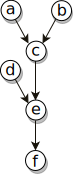
\includegraphics[width=.2\textwidth]{figures/ddg}%
%          \end{figure}
%          \captionof{subfigure}{DDG}
%          \label{fig:ddg_graph}
%      \end{minipage}
%\captionof{figure}{Example DDG with corresponding assembly code.}
%\label{fig:ddg}
%\end{minipage}
%\end{center}
%TODO: add more abstractions, also include dominator tree
Figure \ref{fig:ddg_graph} shows a data dependence graph corresponding to the code fragment in Figure \ref{fig:ddg_fragment}. In a data dependence graph nodes represent operations and the edges correspond to data dependencies.

%========= Store listing box =====
\newsavebox{\ddgfragmentlst}
\begin{lrbox}{\ddgfragmentlst}
  \begin{lstlisting}
(a) lw  r2, r5,  4
(b) lw  r3, r6,  6
(c) mul r3, r3, r2
(d) lw  r4, r7,  0
(e) add r4, r3, r4
(f) sw  r4, r11, 0
  \end{lstlisting}
\end{lrbox}

\begin{figure}[H]
  \centering
  \subfloat[Assembly fragment]{%
%    \usebox{\ddgfragmentlst}\label{fig:ddg_fragment}
   \includegraphics[width=.25\textwidth]{figures/ddg_fragment}\label{fig:ddg_fragment}
  } \quad\quad%\hfill%\hspace{35px}
  \subfloat[DDG]{%
   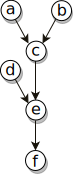
\includegraphics[width=.1\textwidth]{figures/ddg}\label{fig:ddg_graph}
  }
  \caption{Example DDG with corresponding assembly code.}
  \label{fig:ddg}
\end{figure}


%new TODO: add live interval analysis information or theory!!!
%TODO: add sentence in between
Sometimes there are not enough registers available to allocate physical rezgisters to all virtual registers because there are only a limited number of physical registers available. When the compiler runs out of registers to allocate, \emph{spilling} may be necessary to free one or more registers by storing them on the stack. Consequently, it is required to retrieve them from the stack just before they are used.

%TODO: add illustration of spilling?

%todo add theory, graph coloring on ddg graph.


%TODO: add control flow dependecy explanation, optionally from Code Generation for TTAs p.
%TODO: play with widths to get nicely in teh middle of the page.
%\lstset{style=customc}
%\begin{center}
%\begin{minipage}{\linewidth}
%\centering
%\begin{minipage}{0.2\linewidth}
%\begin{lstlisting}
%
%int foo(int z) {
%  x = z-2;
%  y = 2*z;
%  if (z < 0) {
%    x++;
%    y++;
%  } else {
%    x--;
%    y--;
%  }
%  z = x+y;
%  return z;
%}
%\end{lstlisting}
%\end{minipage}
%\hspace{0.05\linewidth}
%\begin{minipage}{0.4\linewidth}
%\begin{figure}[H]
%\centering
%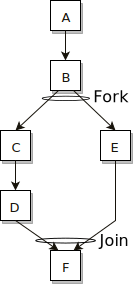
\includegraphics[width=.35\textwidth]{figures/cfg_fork_join}%
%\end{figure}
%\end{minipage}
%\captionof{figure}{A fragment of C code with a CFG.}
%\label{fig:cfg}
%\end{minipage}
%\end{center}

%TODO: insert general RA algorithms and heuristics. Graph colouring, and use this reference \cite{ra}.
%There are multiple register allocators available in LLVM, e.g. basic, fast, greedy and Partitioned Boolean Quadratic Problem (PBQP) register allocation. PBQP is a nearly optimal approach that does register allocation in phases, i.e. spilling, register assignment and copy coalescing. After spilling, RA can be done in polynomial time, but copy coalescing is NP-complete \cite{pbqp}. The other three register allocators are linear scan based algorithms that use heuristics and visit live ranges in order, although it is possible to implement a custom register allocator.
%TODO: decide to add or not to add.

%TODO: insert scheduling talk, including algorithms, heuristics and LLVMs available schedulers.
%TODO: move to later.
%A common problem in compilers is the ordering in which to do scheduling and register allocation. If registers are allocated before scheduling, the resulting code tends to have many storage dependencies that limit code scheduling. On the other hand, if the code is scheduled before register allocation, the schedule created may require so many registers that register spilling is required, which may negate the advantages of instruction-level parallelism (ILP) \cite[Chapter~10.2.4]{dragon_book}. Whether to do register allocation first, or scheduling first, or to address these problems at the same time is often referred to as, phase-ordering problem. 

%In general, you can solve scheduling exactly using algorithms, e.g. integer programming or constraint programming, or one can solve the problem, but without guaranteeing that an optimal solution is found using heuristics. With LLVM there are two main schedulers, i.e. list scheduler and Machine Instruction (MI) scheduler that use heuristics to find a solution, although it is possible to implement a custom scheduler for an architecture at hand. 

%TODO: add basic introduction to bypassing, from presentation.

\newpage
\section{Explicit Datapaths}\label{sec:datapaths}
Data goes through a particular path through the pipeline of a processor and typically, a pipeline is split up in multiple stages. With a lockstep processor, each of the stages are effectively working in parallel. Figure \ref{fig:pipelining} illustrates hardware pipelining for a \emph{Reduced Instruction Set Computer} (RISC) processor. The pipeline is split up in four or more stages, e.g. instruction fetch, instruction decode, execution and write-back stage. During the \emph{instruction fetch} (IF stage) an instruction is loaded from \emph{instruction memory} (IMEM), which is decoded in the \emph{instruction decode} (ID) stage where the type of operation is determined by the opcode and operands are identified by their register addressing, and finally, the operation is executed and the result is written back to the register file.

\begin{figure}[H]
\centering
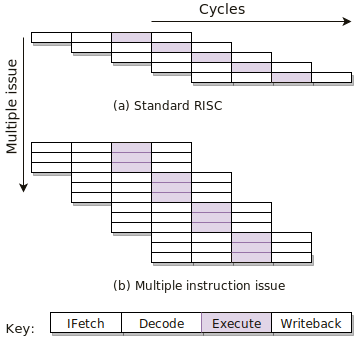
\includegraphics[width=.5\textwidth]{figures/pipelining}
\caption{Pipelining and multiple instruction issue\cite{tta_codegen}.}
\label{fig:pipelining}
\end{figure}

\begin{figure}[b]
\centering
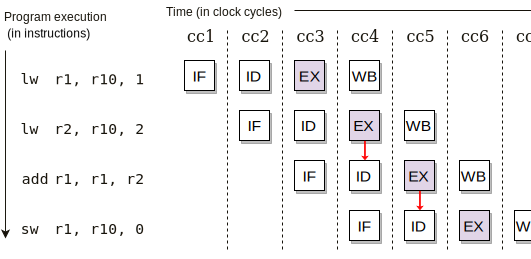
\includegraphics[width=.8\textwidth]{figures/bypassing_example}
\caption{Instructions being executed using the single-cycle datapath, assuming pipelined execution.}
\label{fig:bypass_problem}
\end{figure}

\textbf{Operand forwarding:} When bypassing is completely absent the result of an instruction can only be obtained after it is written back. On the other hand, with bypassing, a bypass network of wires and busses connects the execution and writeback stages back to the ID stage. These wires and busses may be used to forward a value to operands of another instruction. This way, the result of an instruction can be obtained before it has been written back to the register file. This behaviour is illustrated in Figure \ref{fig:bypass_problem}.

Four consecutive instructions are executed of which the last two instructions have a RaW dependency with the instruction prior to it. As you can see in Figure \ref{fig:bypass_problem} the instructions prior to said instructions are in the execution stage when their result is queried, namely, when said instructions are in the ID stage. So either the processor needs to be stalled for a cycle, such that the previous instruction is in the WB stage, or the result needs to be forwarded from the execution stage to the ID stage. Since insertion of stall cycles result in less efficient code, the result is forwarded using the bypass network (indicated with a vertical arrow from EX to ID).

%TODO: update picture, make nicer and have on top stages, and below remain almost the same
%\begin{figure}[H]
%\centering
%\subfloat{\includegraphics[width=.275\textwidth]{figures/bypass_prob_legend}}
%\hfil
%\subfloat{\includegraphics[width=.475\textwidth]{figures/bypass_problem}}
%\caption{Bypassing network differences between four stage and five stage pipeline configuration.}
%\label{fig:bypass_problem}
%\end{figure}
%TODO: replace with picture from presentation (03_nov)
\subsubsection{Implicit Datapaths}
With implicit bypassing (also called transparent bypassing), bypassing opportunities are detected and controlled by dedicated hardware on chip. However, doing this at run-time has some advantages and some disadvantages.
\begin{itemize}
  \item\textbf{Advantage:} 
    With bypassing, operand forwarding is possible which reduces the number of reads from the register file. This will reduce register file usage and may improve energy efficiency of the processor.
  \item\textbf{Disadvantage:} 
    If you push the responsibility of identifying and exploiting forwarding to the hardware, it needs $2\cdot d\cdot n$ comparators (where $d$ is the number of stages between ID en WB and $n$ the number of issue slots) to compare operands of an instruction to registers defined by previous instructions that are already in the pipeline. Altogether, this results in a more complex gate design and increased area.
\end{itemize}

It has been observed that variables in the register file are often transient, meaning that they last only for a short time.  Reads from the register file of said variables can be avoided by forwarding which is shown in the previous paragraphs.\\

Now, we show that register writes of transient values can be avoided with explicit datapaths. The reason why this is only the case for explicit datapaths, and not with implicit bypassing, is that the hardware can only look at instructions that have already been executed, while the compiler can look at all instructions of a program.\\

\textbf{Dead result elimination:} 
If all consumers of a variable obtain it using forwarding, then it will never be read from the register file. Therefore, that variable does not need to be stored in a register file, since it is not read from it anyway. Hence, these obsolete stores may be avoided.  

\subsubsection{Explicit Datapaths}
With explicit datapaths (sometimes referred to as exposed datapaths), bypass opportunities are detected and controlled by the compiler. Doing this at compile time rather than run-time has some advantages and some disadvantages.
\begin{itemize}
  \item\textbf{Advantage:}
    With explicit bypassing, dead result eliminations is possible which reduces the number of writes to the register file. This will further reduce register file usage and may further improve energy efficiency of the processor.
  \item\textbf{Disadvantage:}
    The compiler needs to take datapaths and variables that are in the pipeline into consideration, because bypassing is explicit in the compiler. This results in a more complex compiler.
\end{itemize}

This project focusses on implementing these optimizations for a compiler that targets a wide SIMD architecture. The following section is devoted to explaining the target SIMD architecture.

\newpage
\section{SIMD Processor Architecture}\label{sec:simd}
%TODO: rewrite
%TODO: reduce total number of todos
%TODO: add paragraph about xetal-pro from preparation

The advantage of the SIMD architecture is that multiple operations are processed in parallel instead of sequentially. Therefore, the required throughput can be achieved at a substantially lower clock frequency and thus lower voltage, thereby greatly reducing voltage and thus energy consumption \cite{dongrio1}. Furthermore, because each \emph{Processing Element} (PE) executes the same instruction, the \emph{Instruction Fetch} (IF) and \emph{Instruction Decode} (ID) can be shared among the PEs. Therefore, the area and energy consumed by these parts is negligible.  %Altogether, this results in an ultra-wide SIMD architecture with a high energy efficiency.

A wide SIMD architecture \cite{simd} performs wide vector operations that exploit \emph{Data Level Parallelism} (DLP) by executing the same instruction on multiple data simultaneously. Figure \ref{fig:simd_overview} shows a general overview of the SIMD processor.
There is a \emph{Control Processor} (CP) responsible for the control flow and scalar operations, and there is a wide array of PEs that execute in parallel with the CP, which are responsible for processing vector operations.

\begin{figure}[H]
\centering
\includegraphics[width=.6\textwidth]{figures/simd_overview}
\caption{General overview of the wide SIMD architecture.}
\label{fig:simd_overview}
\end{figure}
A SIMD instruction word encodes two sub instructions, hence it resembles a 2-issue VLIW instruction word. Each sub instruction can generally be any instruction defined in the \emph{Instruction Set Architecture} (ISA). The proposed architecture has a \emph{Reduced Instruction Set Computer} (RISC) ISA and is divided up into three categories of instructions. The list of instructions can be found in Appendix \ref{appendix:isa}. In general, a instruction has three operands of which one destination register and two source operands. A Register-type (R-type) instruciton takes two registers as source operands. Instructions that take one register and a constant immediate as operands are called Immediate-type (I-type) instructions. Finally, the control flow can be manipulated by modifying the program counter using Jump-type (J-type) instructions, which can be executed only by the CP.
\\

In order to support a configurable number of PE elements, a neighbourhood network topology is used for its scalability. With a circular neighbourhood network topology, the connection between the first and last PE does not introduce extra long wires, because the PEs can be placed in a circular manner \cite{dongrio2}.

%As an extra challenge for the compiler, the architecture is designed to be configurable, e.g. width of the PE array, bit width of the wires and registers, the number of stages that the instruction pipeline consists of, and whether it has implicit or explicit bypassing, can be configured. The data width of the wires and registers can be configured into 16-bits or 32-bits.

%A SIMD instructions word encodes two sub instructions, so it resembles a 2-issue VLIW instruction word. Each sub instruction 

%TODO: add here that we have in general an iF, ID, one or more EX and a wb stages and that normally the result is not available until after the wb stageis complete, but with bypassing, whether it is transparent or explicit bypassing, we can get the result at an earlier stage. %TODO: make new pictures for difference 4 and 5 stage without all difficult information


%=============================== NN speech ===============================
%\section{Neighbourhood Network}\label{sec:nn}
%Each processor (CP or PE) does not only execute independently, but can also exchange data with its direct neighbours. However, because we have limited connectivity, moving data from one PE to another PE can introduce additional cycles. Namely, when communicating with non-direct neighbours. The circular neighbourhood network that is used to connect the processors is illustrated in Figure \ref{fig:neighborhood_network}. The CP can select data from the first and last PE, and each PE can communicate with its direct neighbours, or (not illustrated in Figure \ref{fig:neighborhood_network}) receive data from the CP by means of a broadcast.

%\begin{figure}[H]
%\centering
%\includegraphics[width=.4\textwidth]{figures/neighborhood_network}
%\caption{Illustration of the circular neighborhood network.}
%\label{fig:neighborhood_network}
%\end{figure}

%The processor selects data from its neighbours in the instruction decode stage. Depending on the "select data" bits, it either takes data from one of its neighbours or from itself. Table \ref{table:select_data} gives an overview of the communication mode, depending on the value of "select data". The "select data" bits are decoded in each instruction, as we will show in Chapter \ref{sec:isa}.
 
% \begin{table}[H]
%\caption{Communication model for the CP and PEs, depending on the value of "select data".}
%\begin{center}
%\begin{tabular}{|c|c|c|}
%\hline
%\textbf{select data} & \textbf{CP} & \textbf{PE} \\ \hline
%2'b00 & Select data from \emph{self}. & Select data from \emph{self}. \\ \hline
%2'b01 & Select data form \emph{last} PE. & Select data from \emph{right} neighbour. \\ \hline
%2'b10 & Select data from \emph{first} PE. & Select data from \emph{left} neighbour. \\ \hline
%2'b11 & Not used. & Select data from CP \emph{broadcast}. \\ \hline
%\end{tabular}
%\end{center}
%\label{table:select_data}
%\end{table}%

%The processors communicate with each other by writing directly to the output of the operand register based on the values of bits "select data" bits. When the value of these two bits is $00$, data is selected from the processor itself. When these bits are $01$, data is selected from the last PE, in case of the CP executing this instruction, and from the right neighbour in case of a PE executing this instruction. Similarly, having a value of $10$, data is selected from the first PE in case of the CP executing this instruction, or left neighbour in case of a PE is executing this instruction. Finally, a value of $11$ will select data from the CP broadcast in the case that a PE is executing the instruction.


\begin{figure}[t]
\centering
\subfloat[4-stage pipeline processor overview.]{\includegraphics[width=.475\textwidth]{figures/4-stage_bypass}%
\label{fig:4_stage}}
\hfil
\subfloat[5-stage pipeline processor overview.]{\includegraphics[width=.475\textwidth]{figures/5-stage_bypass}%
\label{fig:5_stage}}
\caption{Bypassing network differences between the four-stage and the five-stage pipeline.}
\label{fig:datapath_pipeline_conf}
\end{figure}

%=============================== Datapath speech ===============================
\subsection{Processor Pipeline and Datapath}\label{sec:processor}
%TODO: Write new paragraph about.general layout

Generally, each processing unit (CP or PE) has its own registers and three functional units, i.e. ALU, MUL and LSU. 

The instruction pipeline is divided up into four or five stages. Top down, there is an IF-stage, an ID-stage, one or two execution stages and a Write Back (WB) stage, like traditional lockstep RISC processors. The architecture shown in Figure \ref{fig:4_stage} has four stages while the architecture shown in Figure \ref{fig:5_stage} has five stages.\\

The neighbourhood communication network is implemented by overriding \texttt{operand 1} in the ID-stage. Depending on the decoded instruction, data is selected from another (neighbouring) processing unit, from the local RF or from the bypass network. Each FU has private input registers, which keep the result at the output of a compute unit valid as long as no new operation or input is assigned to it \cite{dongrio1}. This \emph{operand isolation} reduces toggling in the FUs, and creates extra opportunities for bypassing. The outputs can be forwarded using the bypass network to operands of another instruction.

\begin{figure}[b!]
\centering
\subfloat[Datapath with implicit bypassing.]{\includegraphics[width=.445\textwidth]{figures/transparent_bypass}%
\label{fig:transparent_datapath}}
\hfil
\subfloat[Datapath with explicit bypassing.]{\includegraphics[width=.445\textwidth]{figures/explicit_bypass}%
\label{fig:explicit_datapath}}
\caption{Bypassing network differences between implicit and explicit bypassing.}
\label{fig:datapath_approaches}
\end{figure}

The SIMD can be configured to have either implicit or explicit bypassing. With implicit bypassing, also called transparent bypassing it is the hardware's responsibility to handle bypassing. With explicit bypassing, on the other hand, the bypasses are encoded in the instructions, and it is thus the compiler's responsibility to handle bypassing.

%We can configure the SIMD to have four or five stages. With four stages shown in Figure \ref{fig:4_stage}, all instructions take a single cycle, while with the five stages shown in Figure \ref{fig:5_stage}, ALU takes a single cycle, while MUL and LSU take two cycles, as shown in Table \ref{table:FU_cycles}. With 5 stages, MUL takes twice as many cycles. However, additions are simpler to perform, therefore the efficiency. 

%\begin{table}[H]
%\caption{Cycles per FU.}
%\begin{center}
%\begin{tabular}{|c|c|c|}
%\hline & \multicolumn{2}{c|}{\textbf{Cycles}} \\ \hline
%\textbf{FU} & \textbf{4-stage} & \textbf{5-stage} \\ \hline
%ALU & 1 & 1 \\ \hline
%MUL & 1 & 2 \\ \hline
%LSU & 1 & 2 \\ \hline
%\end{tabular}
%\end{center}
%\label{table:FU_cycles}
%\end{table}

%The main difference between the two approaches is that where transparent bypassing always performs a write to a register, this is optional for explicit bypassing, as we will show in Chapter \ref{chapter:software_bypassing}.
Explicit bypassing has as main advantage that certain writes to a register can be avoided. Namely, when the result of an instruction is bypassed and not used anywhere else, it does not need to be stored in a register (\emph{dead result elimination}, Chapter \ref{sec:datapaths}). Avoiding writes to the RF reduces the total energy consumption. Since there are many register files in a wide SIMD, reducing the energy consumption of the register file has a large impact on the overall energy consumption \cite{dongrio1}. Because of this, reducing the register file's energy consumption is of great importance. Furthermore, the explicit datapath shown in Figure \ref{fig:explicit_datapath} has two extra sources compared to the implicit datapath in Figure \ref{fig:transparent_datapath}. These additional bypass sources increase the chance that a result is being bypassed. In the explicit bypassing version, bypassing sources are directly accessible by the instruction. This is done by reserving part of the RF address space for the bypass sources. The disadvantage of this is that the register index space is reduced, however, the instruction format does not require changes in order to encode that an operand comes from the bypass network. (Chapter \ref{sec:design_decisions}). 

The total number of registers grows linearly with the number of PEs because each processor has 32 registers. Hence, a wide SIMD has in total many registers that consume a considerable amount of energy. Namely around 34.6\% of the total energy consumption \cite{dongrio1}. Therefore, 

%Todo: change this picture to have explicit and implicit bypassing instead. State then that we will be focussing on explicit bypasisng.



%Todo: add small example, having on one side normal ops. On the other hand haing implicit bypassing and finally explicit bypassing (without the store).

%\begin{figure}[b!]
%\centering
%\subfloat[4-stage pipeline with explicit datapaths.]{\includegraphics[width=.4\textwidth]{figures/4-stage_bypass}%
%\label{fig:4stage}}
%\hfil
%\subfloat[5-stage pipeline with explicit datapaths.]{\includegraphics[width=.34\textwidth]{figures/5-stage_bypass}%
%\label{fig:5stage}}
%\caption{The pipeline of the SMD processor architecture with explicit datapaths.}
%\label{fig:pipeline_stages}
%\end{figure}

%%=============================== instruction format speech ===============================
%\section{Instruction Format}\label{sec:isa}
%%Change (optional)
%%% namely, one scalar and one vector instruction.
%%With
%%% namely, one scalar instruction that is executed on the CP, and one vector instruction that is executed on each of the PEs.
%Similar to a 2-issue VLIW instruction, an SIMD instruction consists of two subinstructions. An SIMD instruction is a 56-bit instruction that is divided up in two 28-bit subinstructions, namely, a scalar and a vector instruction. Only the CP can perform jump and branch instructions, therefore, the vector instruction can be either a R-type or an I-type instruction, while a scalar instruction can be a R-type, I-type or J-type instruction. Both sub instructions have a format, as shown in Figure \ref{fig:instruction_format}.

%\begin{figure}[H]
%\centering
%\includegraphics[width=\textwidth]{figures/instruction_format}
%\caption{Generic overview of the instruction format.}
%\label{fig:instruction_format}
%\end{figure}

%There are two guard bits $p1$ and $p2$, that can be set by using a set flag instruction. Consequently we can them for predicate execution. The instructions, branch if flag (not) set and conditional move read the predicate flag before executing. For the full overview of supported instructions, see Appendix \ref{chapter:supported_operations}.

%Note that the "select data" bits are also part of the instruction as we explained in Chapter \ref{sec:nn}. The CP and PEs can communicate by setting these bits. The communication model is shown in Table \ref{table:select_data}.







%Mention SoC?

%TODO: add risc or cisc / software pipelining / DSP,Microcontroller or microprocessor / other comp arch?


%Talk a bit about different computer architectures (include software pipelining) and that each of these architectures have different charactaristics and that to see if an architecture is efficient, we need a compiler when designing such architecture to see if it is actually efficient. Introduce llvm then go to next section

%TODO: add computer architecture intro and the need for a wide variety of compilers.
%TODO: add introducing text to answer the question, why do we use LLVM

% move? architecture/compiler down after first couple of chapters

%TODO: elaborate delay slot, with link to explanation of pipelining.
%todo update extend rewrite

\section{Related Work}\label{sec:related_work}

% Other exposed or explicit datapath architectures and their corresponding compilers.

% Other pure SIMD architectures, GPU and its difference if i know this and can tell it.

% Liu's work on compiler design, and what it lacks, proper support for 5-stage configuration, explicit bypass conf. 

%Old rel. work
There is related work for compilers that target SIMD architectures, in particular, a compiler has been developed, referred to as legacy compiler. Furthermore, there is related work in building an LLVM backend, and compiling with explicit datapaths has been an active research topic for other architectures.
% scrap
%The related work is introduced in this part, including the legacy compiler, building the LLVM back-end for SIMD architecture, explicit datapaths in other architecture and some scheduling and register allocation algorithms applied in other compilers.

%\section{Building an LLVM back-end}
%Our backend is derived from tricore tutorial on creating a new backend for the LLVM compiler framework \cite{tricore}. Furthermore, based on that work, an LLVM backend for SIMD architecture without explicit bypassing has been developed \cite{liu_zhenyuan}. However, the current compiler generates code with implicit bypassing. We, therefore, need to extend this to efficiently generate code for explicit bypassing as well. Therefore, our work will be an extension to previously noted work.

\subsection{Other Exposed/Explicit Datapath Architectures}\label{sec:other_explicit_datapaths}
Compiling with explicit datapaths has been an active topic of research. Several architectures that face similar challenges have been investigated. 

%Johan janssen & ... TTA work
%Other exposed datapaths

\subsubsection{Transport Triggered Architectures}\label{sec:tta}
One of the main works that was investigated is the  \emph{Transport Triggered Architecture} (TTA) which has been developed in the MOVE project \cite{tta_codegen}. For TTA architectures, instructions consist of transports that specify the datapath. The difference between TTAs and traditional operation triggered architectures is that TTA are transport driven, hence its name. 

Figure \ref{fig:tta} illustrates how function units and register files are connected to an interconnect network which are programmed by instructions. Programming a TTA consists of moving operands to the input registers of a FU.

\begin{figure}[b!]
\centering
\includegraphics[width=.8\textwidth]{figures/tta_structure}
\caption{General structure of a TTA with interconnect network driven by data transports.}
\label{fig:tta}
\end{figure}

%\lstset{style=customasm}
\begin{lstlisting}
add r1, r2, r3  # r1 = r2 + r3
sub r4, r2, 6   # load from memory at location 0x5
sw  r4, r1, 0   # store r4 at address r1
\end{lstlisting}

First step is to translate each $n$-operand $m$-result operation into $n+m$ moves (so called $n$ \emph{operand moves} and $m$ \emph{result moves}). \texttt{O1} and \texttt{O2} are input ports of the FU and \texttt{R} indicates the output (result) of a FU.
%Insert more text explaining both fragments above and below this paragraph.

\begin{lstlisting}
r2 -> O1add ; r3 -> O2add ; Radd -> r1
r2 -> O1sub ; r6 -> O2sub ; Rsub -> r4
r1 -> O1sw  ; r4 -> O2sw
\end{lstlisting}

Let us assume that there are two FUs named \texttt{alu1} and \texttt{alu2} for ALU operations, and one FU named \texttt{ls} for load-store operations. The suffixes `\texttt{alu1}', `\texttt{alu2}', and `\texttt{ls}' indicate the FU on which the operation is executed.
If the above fragment would be scheduled such that the distance between the final operand and a corresponding result move should be at least the latency of the FU. Then the following (TTA assembly) code may be obtained:

\begin{lstlisting}
r2 -> O1add.alu1 ; r3 -> O2add.alu1 ; r2 -> O1sub.alu2 ; r6 -> O2sub.alu2
Radd.alu1 -> r1  ; Rsub.alu2 -> r4
r1 -> O1sw.ls    ; r4 -> O2sw.ls
\end{lstlisting}


\textbf{Bypassing:} The outputs of the add and subtract operations can be directly moved to the load-store unit. This reduces the schedule by one cycle, however, the number of moves does not change.

\begin{lstlisting}
r2 -> O1add.alu1; r3 -> O2add.alu1; r2 -> O1sub.alu2    ; r6 -> O2sub.alu2
Radd.alu1 -> r1 ; Rsub.alu2 -> r4 ; Radd.alu1 -> O1sw.ls; Rsub.alu2 -> O2sw.ls
\end{lstlisting}

\textbf{Dead result move elimination:} Next it may occur that the values in \texttt{r1} and \texttt{r2} are not live anymore because they are used only once. In that case corresponding moves can be skipped. This gives the following schedule:

\begin{lstlisting}
r2 -> O1add.alu1 ; r3 -> O2add.alu1 ; r2 -> O1sub.alu2 ; r6 -> O2sub.alu2 
Radd.alu1 -> O1st.ls ; Rsub.alu2 -> O2st.ls
\end{lstlisting}

The optimizations that is discussed here for TTA also apply on a wide SIMD architecture, which is discussed in Section \ref{sec:datapaths}. However, their approach can not be used because the SIMD architecture is an operation triggered architecture, data transports are a given. More information on explicit bypassing for TTAs can be found in the work of Hoogerbrugge et. al. \cite{tta, tta_codegen}.

%TODO read chapter 7 and cite to it, add words about TTA compiler. Then can be used yes/no

\begin{figure}[b!]
\centering
\includegraphics[width=.65\textwidth]{figures/vliw_forwarding}
\caption{Block diagram of VLIW architecture with bypassing.}
\label{fig:vliw}
\end{figure}

\subsubsection{Very Long Instruction Word Architectures}
The \emph{Very Long Instruction Word} (VLIW) architecture is designed to optimize \emph{Instruction Level Parallelism} (ILP) by executing multiple instructions in parallel.
Although RISC architectures take advantage of temporal parallelism by using hardware pipelining (explained in Chapter \ref{sec:datapaths}), VLIW architectures take advantage of spacial parallelism by using multiple functional units to execute several operations concurrently. 

Figure \ref{fig:vliw} shows a generic block diagram of a VLIW machine that has multiple instruction issues (three in this example), and each issue has its own decode stage and functional units. The figure also illustrates how the bypass network connects the outputs of the FUs back to the ID stage, allowing results to be forwarded. For VLIW architectures, the complexity of the bypass network grows linearly with the size of the instruction word. Furthermore, traditionally the register file requires $n$ write and $2n$ read ports, where $n$ is the length of the instruction word. This may require a more hungry register file as the power efficiency degrades when increasing the number of ports on the register file \cite{compiler_driven_power_opt}. However, this requirement can be relaxed by clustering, where each cluster may have a dedicated register file, which is often done in modern VLIW architectures.\\

A reconfigurable VLIW architecture is developed in the $\rho$-VEX project at the University of Technology in Delft \cite{p-vex}. This architecture also considers explicit bypassing and other configurable design options, e.g. configurable issue-width, functional units and bit-width of the data.

However, their implementation can not be used because (i) they are using a gcc based compiler instead of a LLVM based compiler and (ii) not a lot of implementation details have been given in their paper.



%\subsubsection{ReMove}
%Another architecture that exploits explicit datapath architectures is the ReMove architecture \cite{remove}. That work focusses on scheduling for partially connected architectures with explicit datapaths. The ReMove architecture is similar to a VLIW, having multiple FUs, however here they have an interconnect network that connects the FUs to the RF. The scheduling algorithm used in this work can not be used in our work, because similar to the legacy compiler for SIMD, this project has a custom backend, which can not be reused for LLVM. However, the basic principles of the scheduling algorithms proposed in this work are still valid and may be reused for our work.

%\section{Scheduling and Register Allocation}
%First of all, from the existing scheduling algorithms, Swing Modulo Scheduling (SMS) seems to be a suitable scheduling approach. It is a heuristic approach that is able to deal efficiently with software pipelining. Furthermore, it is known for its outstanding performance and low computational cost. The generated schedules are near optimal in terms of initiation interval and register requirements \cite{swingmodulo_paper, swingmodulo_thesis}. We consider this a candidate scheduler to use.

%Furthermore, the following literature discusses register allocation for SSA-based programs that solves coloring problem optimally in quadratic-time optimal by decoupling coloring, spilling and coalescing \cite{ra}. This technique may allow us to implement a custom register allocator that solves the problem in polynomial time.

%Finally, there is another project, called Unison. They solve scheduling and register allocation and other code generation tasks by translating them into combinatorial problems and solve them together with constraint programming \cite{unison}. We consider this a candidate constraint solver to use because it can be easily integrated with LLVM.

\subsection{Legacy compiler}\label{sec:legacy_comp}
S. Dongrui et al. proposed this processor architecture \cite{simd} while attaining his PhD \cite{dongrui}. The target wide SIMD architecture was design during that time and the compiler that was developed then has many issues. To start, the compiler has a LLVM frontend and a mostly in C++ implemented backend which is not according to LLVM standard. Therefore, it requires a frontend based on an old version of LLVM and since its front-end evolves over time, it is preferable to be able to update this to the newest version. \\

With C code applications as input language, the compiler can only compile to non-vectorized (CP only) instructions. To generate vectorized code an effort had been made to take OpenCL code as input language \cite{dongrio2}. However, only a subset of OpenCL is supported. Moreover, compilation does often generate incorrect code, or none at all. \\


In his work he shows that the register file is one of the most frequently used, and most power-hungry components in a processor. Therefore, he introduced an explicit datapath to further improve energy efficiency on this extremely energy efficient processor architecture. Moreover, efficient code generation for such architecture is key to achieve high energy efficiency for the whole processor. For this reason, the efficiency of the generated code is improved by standardizing the compiler to a frequently used framework. Namely, by standardizing to LLVM. This way we may benefit from developments in the field of compilers and from improvements made to the LLVM framework.
%A compiler had already been developed during the design phase of the target wide SIMD architecture \cite{dongrui}. That compiler has an assembler that can translate from assembly to object code and the compiler can translate C code to scalar only- and OpenCL to vectorized assembly code or object code. That compiler consists of a LLVM front-end and the back-end is developed in C++, but not within the LLVM framework.

%The legacy compiler was developed by the ES group in 2003. We will use the SIMD architecture as it was designed during that time . The legacy compiler has a custom backend for the SIMD architecture that can generate code for explicit datapaths \cite{dongrio1}, but it can only compile C code to non-vectorized instructions or a small subset of hand-touched OpenCL code that also requires manual insertion of custom pragmas to compile for vectorized code \cite{dongrio2}. Our goal is to overcome certain limitations and improve the compilers maintainability.
 

%Dongrio's simd work 

\subsection{Basic Compiler Design}\label{sec:basic_compiler_design}
This section explains an initial design of a SIMD back-end designed within LLVM developed by L. Zhenyuan \cite{liu_zhenyuan}. He started to build a back-end in LLVM for the same purpose, but with a different goal, namely how to generate efficient vectorized code within LLVM. In order to support vector instructions, LLVM's auto-vectorizer has been used and intermediate code optimization passes have been implemented to generate SIMD specific intrinsics, that are, in turn, transformed to vector instructions and shuffle operations. 

His work gives a basic design for this back-end that targets a wide SIMD architecture. The compiler that he developed is taken as a starting point, and is maintained, improved and extended which is discussed in later sections. When building a back-end in LLVM, first the instructions and registers have to be defined. Then illegal operations and types can be converted to legal ones. Then during instruction selection, LLVM knows how to match DAG nodes to known instructions. The supported instructions and registers for this architecture are defined first. To support some special features of this architecture, custom passes are added to this back-end, which will be described in detail, see Chapter \ref{sec:code_generation}, where our contributions to this work are discussed. Furthermore, an assembler and a linker have been implemented as separate projects, which will briefly be discussed here as well.

\subsubsection{Supported Instructions}
All the instructions which have been defined in this compiler are listed in this part, with the corresponding brief explanations. The details of ISA can be found in Appendix \ref{appendix:A}.
\begin{itemize}
	\item \textbf{Arithmetic and Logic Instructions:} \texttt{add}, \texttt{addi}, \texttt{sub}, \texttt{muli}, \texttt{mulu}, \texttt{mului}, \texttt{or}, \texttt{ori}, \texttt{and}, \texttt{andi}, \texttt{xor}, \texttt{xori}, \texttt{sll}, \texttt{slli}, \texttt{sra}, \texttt{srai}, \texttt{srl} and \texttt{srli}.\\
The instruction with suffix "I" is used to handle immediate value operand, which is referred to as I-type instructions. The suffix "U" means it is used for unsigned values. For others, the two input operands are both registers, which are commonly referred to as R-type instructions.
	\item \textbf{Flag Set Instructions:} \texttt{sfeq}, \texttt{sfne}, \texttt{sfles}, \texttt{sflts}, \texttt{sfges}, \texttt{sfgts}, \texttt{sfleu}, \texttt{sfltu}, \texttt{sfgeu} and \texttt{sfgtu}.\\
The flag set instructions are used for comparison. If it is true, the flag register is set. The suffix "S" represents a signed value, while the suffix "U" represents an unsigned value.
	\item \textbf{Conditional Move:} \texttt{cmov}.\\ This is usually used with flag set instructions. If the flag is set, the value in the input operand is moved to the output operand.
	\item \textbf{Immediate Extension:} \texttt{simm} and \texttt{zimm}.\\ These two instructions are used to extend the immediate value from 8 bits to 26 bits. The maximum immediate value could be $2^{26}-1$, instead of $2^8-1$. The details of these two instructions will be discussed in Section \ref{sec:immediate_ext}. In addition, a larger immediate value requires a sequence of instructions to be executed.
	\item \textbf{Conditional Branch:} \texttt{bf} and \texttt{bnf}.\\ These two instructions also work with flag set instructions. By using the branch in- structions, the program can branch to the target address if the flag is set (with BF) or not set (with BNF).
	\item \textbf{Jump Instructions:} \texttt{j}, \texttt{jr}, \texttt{jal} and \texttt{jalr}.\\ The difference with the conditional branch instructions is that the jump does not need to check the flag register, which is normally used during function call and return.
\end{itemize}

\subsubsection{Register Configuration}
There are two main register classes. Although each PE has its own register file in our architecture, it is not necessary to define a specific register class for every PE register file. One reason is the size of the PE array is configurable and the number of the vector register classes cannot be dynamic. Another reason is, the vector array actually is a single issue slot, which executes the same instruction for all PEs. It is sufficient to define one register class for the entire PE array. Each vector register defined in the back-end represents a line of registers in the PE array.

\begin{table}[t]
\caption{Registers configuration.}
\begin{center}
\begin{tabular}{@{}l l l@{}}
\toprule
\textbf{Scalar Register} & \textbf{Vector Register} & \textbf{Purpose} \\ \hline
\texttt{r0} & \texttt{v0} & Constant value zero \\
N/A & \texttt{v1} & Constant PE index \\
\texttt{r3}$\sim$\texttt{r4}  & \texttt{v3}$\sim$\texttt{v4} & Return registers \\
\texttt{r5}$\sim$\emph{r8} & \texttt{v5}$\sim$\texttt{v8} & Argument passing registers \\
\texttt{r9} & N/A & Link register \\ 
\texttt{r10} & N/A & Frame pointer \\
\texttt{r11} & \texttt{v11} & Stack pointer \\
\texttt{r1}, \texttt{r2} and \texttt{r12}$\sim$\texttt{r31} & \texttt{v2}, \texttt{v9}$\sim$\texttt{v10} and \texttt{v12}$\sim$\texttt{v31} & General purpose registers \\
\bottomrule
\end{tabular}
\end{center}
\label{table:register_conf}
\end{table}%
%TODO: add text that goes by this, and optionally change lists in tables.

Table \ref{table:register_conf} shows the register configurations of both CP and PE-Array.
Both \texttt{r0} and \texttt{v0} are connected to ground and contain constant value zero. \texttt{v1} is a special register, which contains the index of local PE. Note that, there are two stack pointers, \texttt{r11} and \texttt{v11}. As mentioned before, considering there are two separated data memory, a double frame stack is needed for the CP and PE-Array to access their memories directly and reduce the expensive data communication. Therefore, two stack pointers are defined to point to the top of scalar and vector frame stacks respectively. The details of separate frame stacks is not described here, but can be found in another thesis \cite[Chapter~4]{liu_zhenyuan}.

\subsubsection{Vectorizer}
 Support for LLVM's Auto-Vectorizer has been developed by L. Zhenyuan. He added support for this to our back-end during his time \cite[Chapter~5]{liu_zhenyuan}. He defined a couple of patterns to match and IR level transformations that transform loops to vector instructions and shuffle operations. Furthermore, he added a cost function to decide whether to vectorize a given loop automatically. However, sometimes the auto-vectorizer fails to vectorize a simple loop. In those cases, pragmas are manually inserted directly before a loop in the C code. Clang uses these pragmas for making decisions on whether or not to vectorize a given loop. In the end, this may give better results, as will be shown in Chapter \ref{chapter:evaluation}.
 
 Supported vector types are:
 \texttt{v1i32}, \texttt{v2i32}, \texttt{v4i32}, \texttt{v8i32}, \texttt{v16i32}, \texttt{v32i32}, \texttt{v64i32}, \texttt{v128i32}, \texttt{v256i32}, \texttt{v512i32}, \texttt{v1024i32} and \texttt{v2048i32}.\\
	The actual legal vector type should be equal to or smaller than the \texttt{PENum}. \texttt{PENum} is a variable defined in the back-end, which can be configured using \texttt{pe-num} flag. The default value is 8, in which case the legal vector type can only be \texttt{v1i32}, \texttt{v2i32}, \texttt{v4i32} and \texttt{v8i32}.

\subsubsection{Linker and Assembler}
An assembler has been implemented that can parse assembly code and translate it into binary code. Furthermore, a linker has been developed which takes one or more binary files and combines them into a single executable file. These have been developed as separate projects and within the LLVM framework. Unfortunately, the linker still has some problems that need to be resolved before it can be used. %TODO go deeper into limitations of the lld linker
Therefore, a custom linker is chosen instead of the standard linker supplied by LLVM. We would benefit from using LLVM's linker because the custom linker can work only on a single file. Unfortunately, this linker can not be used yet because it is a work in progress.%work in progress

%TODO: add bypassing, auto and expl, (from slides)

